---
name: TikZ Flowchart
category: diagrams
description: Flowchart with decision and process nodes
packages:
  - tikz
preamble:
  - \usetikzlibrary{shapes.geometric,arrows.meta,positioning}
---
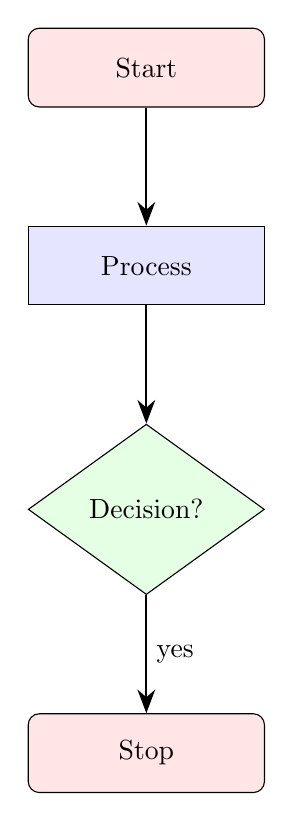
\begin{tikzpicture}[
  startstop/.style={rectangle, rounded corners, minimum width=3cm, minimum height=1cm, draw, fill=red!10},
  process/.style={rectangle, minimum width=3cm, minimum height=1cm, draw, fill=blue!10},
  decision/.style={diamond, minimum width=3cm, minimum height=1cm, draw, fill=green!10},
  arrow/.style={-{Stealth[length=3mm]}, thick},
  node distance=1.5cm
]
  \node (start) [startstop] {Start};
  \node (process) [process, below=of start] {Process};
  \node (decision) [decision, below=of process] {Decision?};
  \node (stop) [startstop, below=of decision] {Stop};

  \draw [arrow] (start) -- (process);
  \draw [arrow] (process) -- (decision);
  \draw [arrow] (decision) -- node[right] {yes} (stop);
\end{tikzpicture}
